%----------------------------------------------------------------------------
\chapter{Railway demonstrator system architecture}\label{chapter:RailwaySystem}
%----------------------------------------------------------------------------
First of all this section describes the railway demonstrator system architecture as it is the system under test.(A top overview of the demonstrator system is shown in \autoref{fig:overview}.) This system's purpose is to simulate a real-life safety critical railway system, with basic functionalities and with a safety logic. The demonstrator is based on a railway model stub which is extended with custom and off-the-shelf hardware and software components. Naturally the system is also capable of moving and stopping the trains on them, nevertheless with the safety logic it can avoid safety-critical scenarios like train collision or train derail. In the following chapter I will further discuss the system architecture with their components and describe the requirements for them.
\begin{figure}[ht]
	\centering
	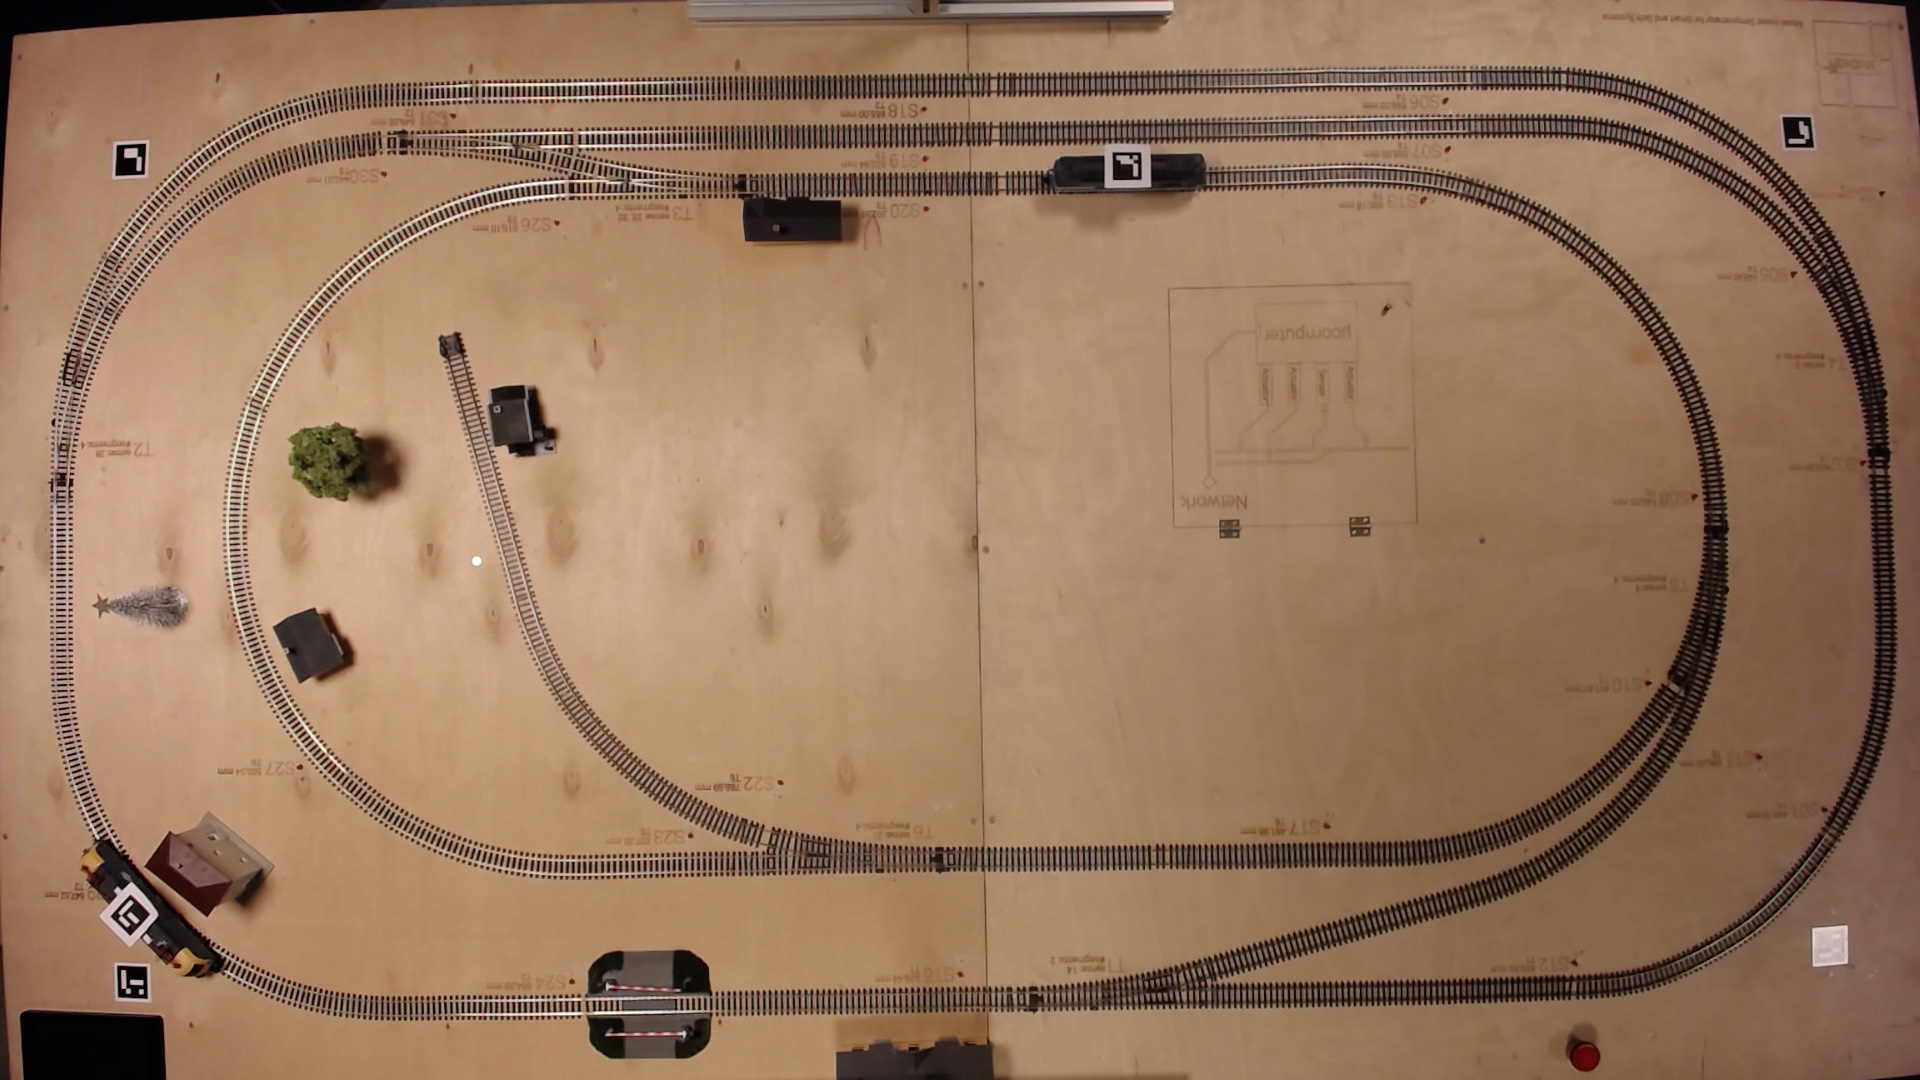
\includegraphics[width=150mm, keepaspectratio, angle = 180]{figures/modes3/overview.jpg}
	\caption{Railway system top view}
	\label{fig:overview}
\end{figure}

\section{Railway system basic components}
I will introduce the physical components and the basic process of the railway systems stub in the following section. Basically there are 31 sections, with one blind track and 7 turnouts. \autoref{fig:layout} shows the layout of railway elements with the corresponding segment ids. In the following, the abbreviation of S is stands for sections and T is for turnouts.
\todo[inline]{Create more visible figure about layout?}

\begin{figure}[ht]
	\centering
	\includegraphics[width=150mm, keepaspectratio]{figures/modes3/layoutBigsmall.png}
	\caption{Railway layout}
	\label{fig:layout}
\end{figure}

\paragraph{Section} 
First principal element is a 30-65 cm long railroad. Each section is connected to 2 other segments (except the S22 blind section) and wired to a command station, which gives them sufficient power source for moving the trains on them. On \autoref{fig:layout}, these sections are identified by \textit{SXX} strings, where \textit{XX} is two unique digits for this layout. Furthermore these numerals determine which bit shows this section's occupancy in the occupancy vector (see section \ref{section:OccupancyDetection} for more information). After the identifier each section lengths are shown with responsible BeagleBone Black ids.

\paragraph{Turnout}
The second principal element is the turnout, which can differentiate 2 paths on the track. The train which is going through a turnout can reach different sections depending on the state of the exact turnout. On the \autoref{fig:turnoutDir} \textit{T1} turnout illustrates a regular turnout and \textit{T3} exemplifies an English turnout. On the layout figure (\ref{fig:layout}) each of these elements are visible as gray dashed sections with the IDs. Each turnout ID starts with T and ends with a numeric (1..6). These IDs determines, which bit identifies the turnout's occupancy in the occupancy vector) and \textit{\#segments} as number of supervised sections by the corresponding BeagleBone Black (see section \ref{section:OccupancyDetection} for more information about occupancy vector). 

\begin{figure}[ht]
	\centering
	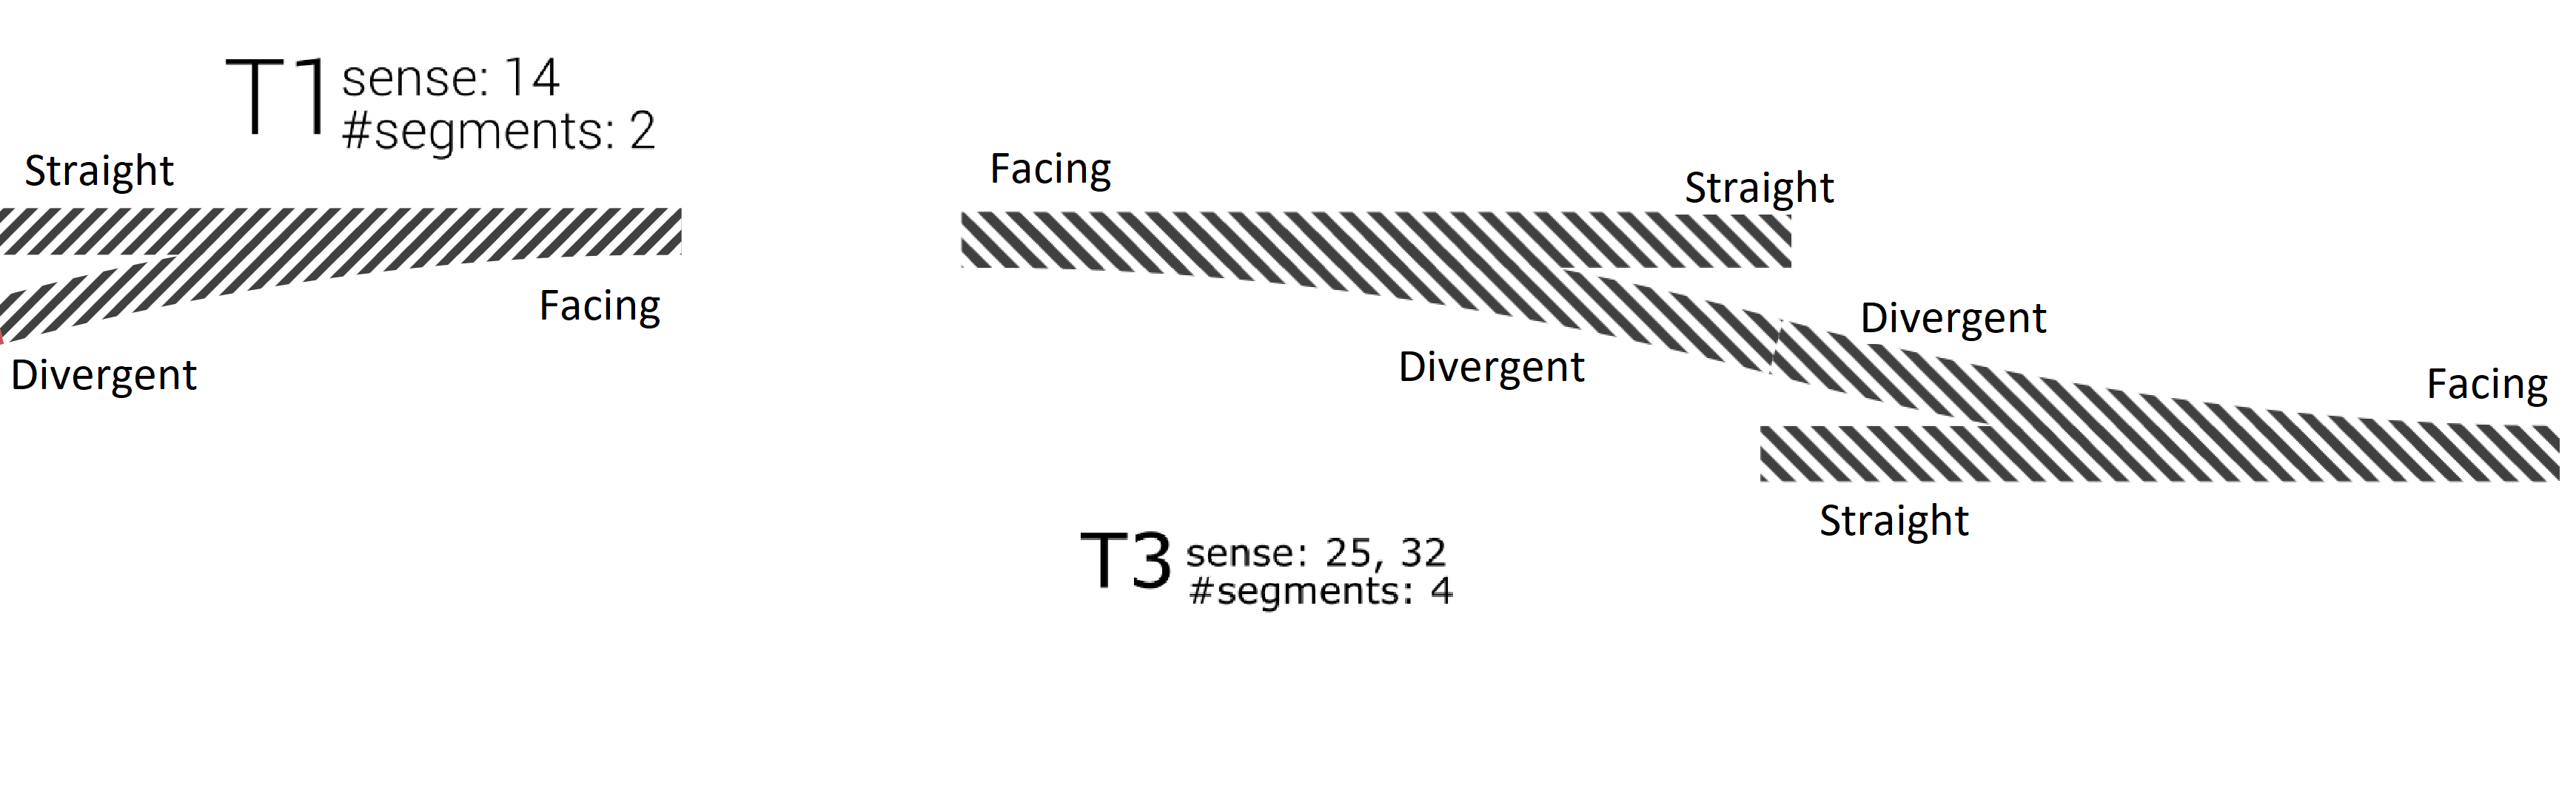
\includegraphics[width=150mm]{figures/modes3/t1andt3.png}
	\caption{Turnout directions}
	\label{fig:turnoutDir}
\end{figure}

\paragraph{Train}
Any model train can be used with the demonstrator system, which can be moved on the track elements. With a supplementary element a train's speed and length can be measured.

\paragraph{Command Station} \label{basics:CS}
Supply power source for the sections which provides tension for the trains on the track. Although an off-the-shelf microcontroller consumes 5V DC, the command station supplies 12V DC. Therefore we have to convert down the power source to match the microcontroller's needs. (For more details see \autoref{par:BBBcape})

\todo[inline]{footnote is ok? move it out to the bibs?}
\paragraph{Controller}
In connection with the \textit{Command Station} an XPressNet protocol \footnote{More details about XPressNet Protocol \url{http://www.lenzusa.com/1newsite1/Manuals/xpressnet.pdf}} based controller is attached to the system. This component's purpose is setting the direction and speed for each train on the track.

\section{Hardware extensions}
The basic hardware environment is not sufficient for controlling and analyzing purposes, therefore additional hardware elements have been designed to satisfy these requirements. In this section these platforms will be described in details. (The \ref{appendix:HWPictures} appendix contains pictures about the elements.)
\todo[inline]{Check if these infos are necessary and where to put them}
For modeling purposes I have used MagicDraw with Sysml plugin \cite{SysML}.

\subsection{Data processing units}
\begin{figure}[ht]
	\centering
	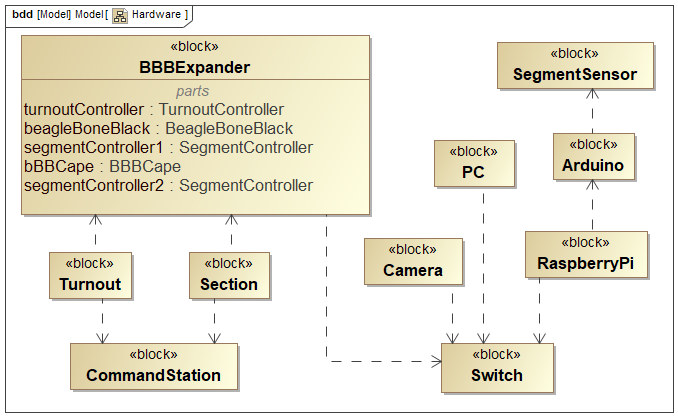
\includegraphics[width=150mm]{figures/modes3/Hardware.png}
	\caption{Hardware block definition diagram}
	\label{fig:Modes3HWBDD}
\end{figure}

\paragraph{BeagleBone Black (BBB)}
An industrial microcontroller platform which provides 4GB 8-bit eMMC on-board flash storage and 2x PRU 32-bit microcontrollers, which could satisfy the function for parallel monitoring. There are 6 BBB on the track connected to the railway, used for controlling turnouts and enabling/disabling each section.

\paragraph{Rapsberry Pi 3}
A Rapsberry Pi microcontroller is dedicated to handle most of the software components related to the Railway demonstrator system. It has twice as large computing capacity in RAM and also in CPU as BBB.

\paragraph{Arduino}
Dedicated hardware element for reading the 6 DigiSens-8-S88 output data through S88 protocol (see \ref{par:SegmentSensor} section for details about this component). This communication layer requires proper timing conditions which the Arduino platform can satisfy.

\paragraph{Camera}
A web camera is placed above the demonstrator table, so it gets a top overview of the table.

\subsection{Custom hardware extensions}\label{section:CustomHW}
\paragraph{BeagleBone Black cape and expanders}\label{par:BBBcape}
The BeagleBone Black components expect 5VDC power source instead of 12VDC which our power station supplies. Because of that reason a so called cape have been created for each controller. Additionally the need for easy-to-use ports to attach additional circuits to the main board also have come up. The expanders could be used to extend the functionality of one BeagleBone unit, which is on the figure \ref{fig:capeSysml}. 

\begin{figure}[ht]
	\centering
	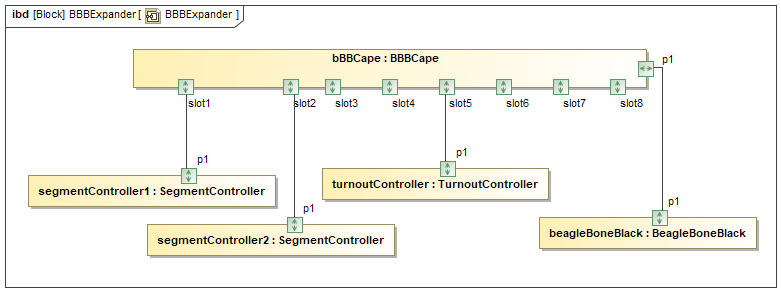
\includegraphics[width=150mm]{figures/modes3/BBBExpander.png}
	\caption{Layout and current attachment of cape and expander}
	\label{fig:capeSysml}
\end{figure}

Each cape have 8 general purpose expander slot, for which the pin layout is expressed in the following \ref{table:expander_pin_layout} table.

\begin{table}[ht]
	\caption{Pin layout}
	\label{table:expander_pin_layout}
	\begin{center}
		\renewcommand{\arraystretch}{1.5}
		\begin{tabu} to 0.5\textwidth { | X[c] | X[c] | X[c] | X[c] |}
			\hline
			pin3 & pin2 & pin1 & pin0 \\ \hline
			3V3  & 5V   & Gnd  & 12V  \\ \hline
		\end{tabu}
	\end{center}
\end{table} 

The upper row of each connector is dedicated for GPIO connections. Two of the GPIO pins connected to the application processor and the remaining two GPIO pins are connected to the PRU unit. With this setup, the PRU and the application processor can cooperate on hardware level.

\paragraph{Segment sensor}\label{par:SegmentSensor}
The DigiSens-8-S88 component is an off-the-shelf product, which can detect the occupancy for 8 segments. \footnote{More information about the product can be found here:\url{http://www.digitools.hu/termekek/erzekelok/digisens-8-s88}}.

\paragraph{Segment actuator}
Segment Actuator expanders are designed to stop a train on the corresponding segment. The concept behind this expander based on the Lenz Asymmetrical DCC and Automatic Brake Control functionality of train-decoders. Every Segment Actuator expander has two slots (A or B) and can enable and disable two segments. Each segment can be enabled setting two GPIOs to HIGH level. One GPIO is connected to the PRU and the other to the application processor.

\paragraph{Turnout actuator}
Turnout Actuator expanders can switch turnouts on the table between their states. Previously a Commercial off-the-shelf (COTS) units was user for this purpose, but in that case we were not able to query the position of a switch programmatically. The Turnout Actuator expander gives the ability for both, switching the turnout and sensing its state.

The concept behind this unit is based on the fact, that turnout mechanism is working as a wire between the common (COM) pole and an other pole (straight or divergent) when switched in one position, therefore we can sense its state.

The electronic characteristics of the BeagleBone unit could not satisfy the switching process electrically, thus we had to use an ATmega328 micro-controller unit (Arduino). Additionally the state-sensing process is based on Analog to Digital Converters, which are also integrated into the Arduino.

For usage, the Arduino has 2 input and 2 output pins connected to the expander connector as shown in the \autoref{table:MCU}. The turnout switching information is input for the Arduino and the turnout state sensing is an output information for that, because it supplies the turnout actuator elements with these details.
\begin{center}
	\label{table:MCU}
	\renewcommand{\arraystretch}{1.5}
	\begin{tabu} to 0.7 \textwidth {X[c] X[c] X[c] X[c]}
		\toprule
		Pin 0    & Pin 1                           & Pin 2    & Pin 3                           \\ \midrule
		Straight & Divergent                       & Straight & Divergent                       \\
		  \multicolumn{2}{c}{Turnout switching}    & \multicolumn{2}{c}{Turnout state sensing}  \\
		\multicolumn {2}{c}{Input for the Arduino} & \multicolumn{2}{c}{Output for the Arduino} \\ \bottomrule
	\end{tabu}
\end{center}

\section{Software components}\label{section:CustomSW}
In general the following software components were implemented in java and c++ languages and deploying separation is shown in \autoref{fig:Modes3Deployment}. Mainly each BBB microcontroller have TrackElementController deployed involving the GPIO, PhysicalSegmentController and PhysicalTurnoutController components. The Rapsberry Pi serves the Dashboard, Touchboard, Messaging and OccupancyQuery components and the Arduino microcontroller is dedicated for SectionOccupancyQuery functionality.

\todo[inline]{delete physical controllers? add xpressnet controller? update figure to be nicer and add componentlevel SL}
\begin{figure}[ht]
	\centering
	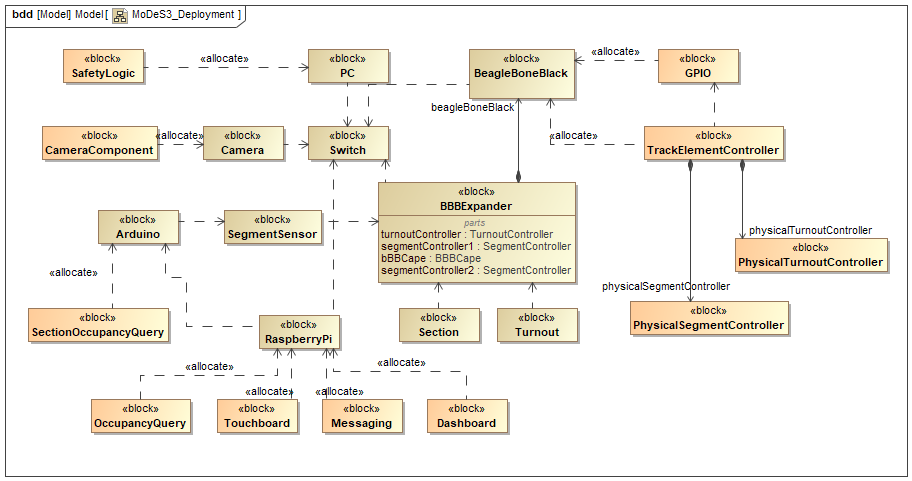
\includegraphics[width=150mm]{figures/modes3/MoDeS3_Deployment1.png}
	\caption{Software components deployment to hardware elements}
	\label{fig:Modes3Deployment}
\end{figure}

\subsection{Occupancy detection elements} \label{section:OccupancyDetection}
\paragraph{Section Occupancy Query}
Responsible for debouncing the 32bit long occupancy vector with proper timing conditions regarding S88 protocol and forward this 32bit to \textit{Occupancy Query} through usb connection. Computed data contains the occupancy information for each track element (section or turnout) per one bit.
\paragraph{Occupancy Query}
In connection with the \textit{Section Occupancy Query}, this component is storing the occupancy states for the whole track. Only if the state has changed for one segment, it sends an occupancy change message to the dedicated MQTT topic with the track element id and the track's new occupancy state.

\subsection{Track segment control elements}
\paragraph{GPIO}
Handles the GPIO pin changes and commands for each extension point of the BBB cape (see \ref{par:BBBcape} section for details about BBB cape and expanders).
\paragraph{Track Element Controller}
On each BeagleBone Black microcontroller there is a controller, which executes the turnout and segment operations for the supervised sections. To satisfy this functionality this controller forwards commands to the corresponding Physical Segment or Turnout Controllers, which communicates with GPIO managers. Consequently with this software component, we are able to enable or disable sections and set turnout directions.

\subsection{Track control and supervisor elements}
\paragraph{XPressNet controller}
Provides a protocol for sending messages to the \textit{Command Station} component, therefore we can extend the communication form for controlling the track. In the current layout there is a controller and a web-based opportunity for controlling also.
\paragraph{Dashboard}
Model railway track dashboard implementation, where we can manipulate the track elements. In Addition this component is instantiated only once, and up for the whole time while the track is in use. Consequently we can reach one common dashboard from the web and it contains the actual occupancy and track element status. It is deployed on the Raspberry Pi microcontroller, which starts the service automatically at startup.
\paragraph{Touch board}
Dashboard for the model railway track, with focus on touchable elements, that can be controlled. This touch board is attached to the demonstrator table itself and start automatically with the Dashboard on the Raspberry Pi microcontroller.
\paragraph{Safety Logic}
In the MODES$^3$ safety-critical project we want to avoid the collision of model trains and the turnout derail scenarios, therefore the safety logic software component detects these critical scenarios by Viatra Query \cite{Viatra} patterns and act the necessary action (for example disable a section or the whole track). The component level safety logic is a light-weight implementation with Gamma Statechart Composition Framework \cite{Gamma}, that also serves this purpose and deployed to each BBB separately.
\todo[inline]{make bib references for viatra, yakindu}

\subsection{Communication topics}
Each software component share informations about the railroad system through the messaging software element, which is based on protobuf messages and provides high-level designed API with MQTT connection for this purpose. 
\begin{figure}[ht]
	\centering
	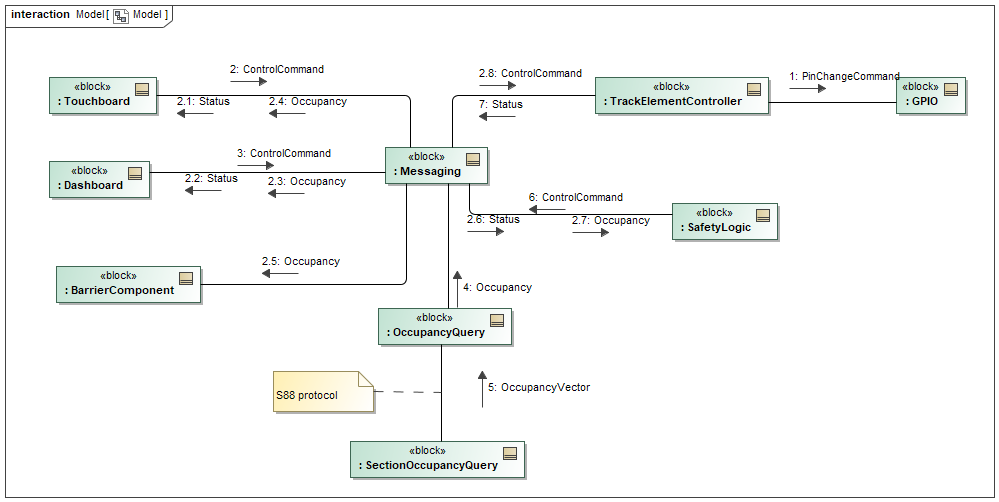
\includegraphics[width=150mm, keepaspectratio]{figures/modes3/CommunicationModel.png}
	\caption{Communication between software components}
	\label{fig:communicationModel}
\end{figure}

Separated topics are distinguished for different information flows, for which any component can subscribe. Basically all topic is change based, therefore every component must send a signal message to the dedicated topic with the proper information of the change like their state have been changed. For example, if a specific section became free, then the \textit{OccupancyQuery} component sends an OccupancyStateChanged message to the Segment Occupancy topic with free state and with the specific section's ID. Although there is a \textit{SendAllStatusCommand} which asks every component to send their actual status with their unique identifier.

In the following paragraphs , I will list the specific MQTT topics and the connected software components. So basically what kind of information is shared on those topics.

\paragraph{Segment Occupancy topic}
On this topic the \textit{Occupancy Query} component sends information whether an occupancy's state is changed on a segment. (Notice that a segment can also be a section or a turnout too.) Most of the components are subscribed for this topic as they want to have information which segment is occupied. These components are the \textit{Touch board}, \textit{DashBoard}, \textit{Barrier} (only for the supervised segments), \textit{Track Element Controller} and \textit{Safety Logic}.

\paragraph{Segment and Turnout Command topic}\label{par:MQTTTopicCommand}
Basically the \textit{Track Element Controller} process and accomplish these commands, and \textit{Touch board}, \textit{Dashboard} and \textit{Safety Logic} components can give these instructions.

\paragraph{Segment and Turnout Status topic}\label{par:MQTTTopicStatus}
For every command the \textit{Track Element Controller} will give a status acknowledgment message with the new state of the turnout or section. In this way the \textit{Touch board}, \textit{Dashboard} and \textit{Safety Logic} elements will be informed about current/new state.

\paragraph{Computer Vision topic}
The camera notification is communicated on that topic, which is received only by the system level \textit{Safety Logic}.

\paragraph{All topic}
For this specific topic all the components in the system are subscribed, and information about train controlling and \textit{Command Station} related messages are shared.

\subsection{Communication messages}
\todo[inline]{some intro needed}
\begin{table}[ht]
	\caption{Message types}
	\label{table:MessageTypes}
	\begin{center}
		\renewcommand{\arraystretch}{1.8}
		\begin{tabu} 
			to 1.0 \textwidth
			{  X[0.6, l] X[l] }
			\toprule
			Message Name                  & Details                                                                           \\ \midrule
			                                      \multicolumn{2}{c}{Command messages}                                        \\
			SendAllStatus                 & Every receiver should send back their information about everything they store   \\
			DCCOperationCommand           & sent via XPressNet protocol by the digital command control (DCC)                  \\
			SegmentCommand                & to enable or disable a specific segment                                           \\
			TrainReferenceSpeedCommand    & to set the speed and direction for a specific train with DCC                      \\
			TurnoutCommand                & to set a turnout into straight or divergent state                                 \\
			                                       \multicolumn{2}{c}{Status message}                                         \\
			ComputerVisionObjectPositions & position details of a physical object on the track                                \\
			DCCOperationState             & actual status information about DCC operation                                     \\
			SegmentOccupancy              & occupied or free status information about a segment                               \\
			SegmentState                  & enabled or disabled status information about a segment                            \\
			TrainReferenceSpeed           & train reference speed status information                                          \\
			TurnoutReferenceState         & straight or divergent status information about a turnout sent by train controller \\
			TurnoutState                  & straight or divergent status information about a turnout                          \\ \bottomrule
		\end{tabu}
	\end{center}
\end{table}

\subsection{Complementary elements}
\paragraph{Barrier} 
Handle commands to open/close the barrier via the network.
\paragraph{Computer vision}
Calculates the coordinates of each elements which have a marker like trains. The position information can be used by the \textit{Safet Logic} to avoid safety-critical scenarios.

\section{Safety-critical functionalities}\label{section:SC-Functionalities}

\todo[inline]{Maybe a figure of the Sw-Hw sysml for each paragraph}

\paragraph{Occupancy detection}\label{par:FunctionOccupancyDetection}
In order to know where are the trains on the track, we first must know which track element (section or turnout) is occupied. This attribute can be determined whether the specific section has power consumption or not, because of a train . The actual detection is made by the \textit{DigiSens-8-S88} sensing element. The demonstration railway system have four sensing elements, and they are connected to an \textit{Arduino} through S88 port. This microcontroller computes basic calculations by \textit{Section Occupancy Query} C++ software component and forwards the 32-bit occupancy vector information (current state of every track element) to the \textit{Occupancy Query} via USB connection. The \textit{Occupancy Query} Java component compares the new occupancy states with the previous one and sends a \textit{SegmentOccupancy} message to the \textit{Segment Occupancy} topic about the change.

\paragraph{Track element controlling}\label{par:FunctionTEC}
For safety-critical purposes, any collision scenario can be avoided by stopping the trains. For this purpose it is a good manner to disable a track element, which is affected in the critical scenario. To make this switch possible, we have to cut the electric circle between the segment and \textit{Command Station}. The \textit{Section Controller} hardware element have been developed for changing a section's state,  the \textit{Turnout Controller} is responsible for changing a turnout's state. These hardware elements are attached to a \textit{BBB cape}, which is designed for extending the ports of BBB. In software point of view, through GPIO pins (specific file writing), we can give impulses from the BBB to the section or turnout. Therefore a \textit{GPIO manager} component is responsible for that in connection with the \textit{Track Element Controller} component. Both of them are Java components and deployed to the BBB microcontrollers.

\paragraph{Safety critical verification}
Because of the network communication, it is easy to connect a \textit{Safety Logic} into the system. In addition a camera (which has a top overview of the table) can read the position of a train on the track. If the \textit{Safety Logic} detects an unsafe scenario with the occupancy detection or camera, it switches off the affected segments or the whole track.

In the demonstrator architecture we can distinguish two different safety logic implementations. First is a component-based approach, which derives each component's scope to the supervised sections of one BBB (as defined in \autoref{fig:layout}). Consequently these elements are deployed to every BBB. The other implementation is a system level safety logic and uses Viatra \cite{Viatra} queries on an Eclipse Modeling Framework (EMF) model to avoid safety-critical scenarios. This model is updated with communication messages thus it observes every topic on the network.

\paragraph{Safety Logic: Turnout derail test coverage items (FS-4/2.0)}
\begin{enumerate}[label=FS-5/2.0-\arabic*, leftmargin=*, format=\small]
	\item Train is moving through a turnout from top to divergent, while the turnout is in straight state
	\item Train is moving through a turnout from top to straight, while the turnout is in divergent state
\end{enumerate}

\section{Safety-critical scenarios}
\todo[inline]{redraw?}
\paragraph{Train collision scenarios} 
To avoid any train collision on a track, it is necessary to measure the distance between the trains. In the demonstrator railway system, we can measure the position so as well the distance between to trains by using the segment occupation information or with the \textit{Computer Vision} component. 

Let's consider an example case (shown in \autoref{fig:LayoutT1-scenario1}), where \textit{Train 1} is going to the section where \textit{Train 2} is staying. Notice that no matter in which direction the \textit{Train 2} is moving this is an unsafe situation.
\begin{figure}[ht]
	\centering
	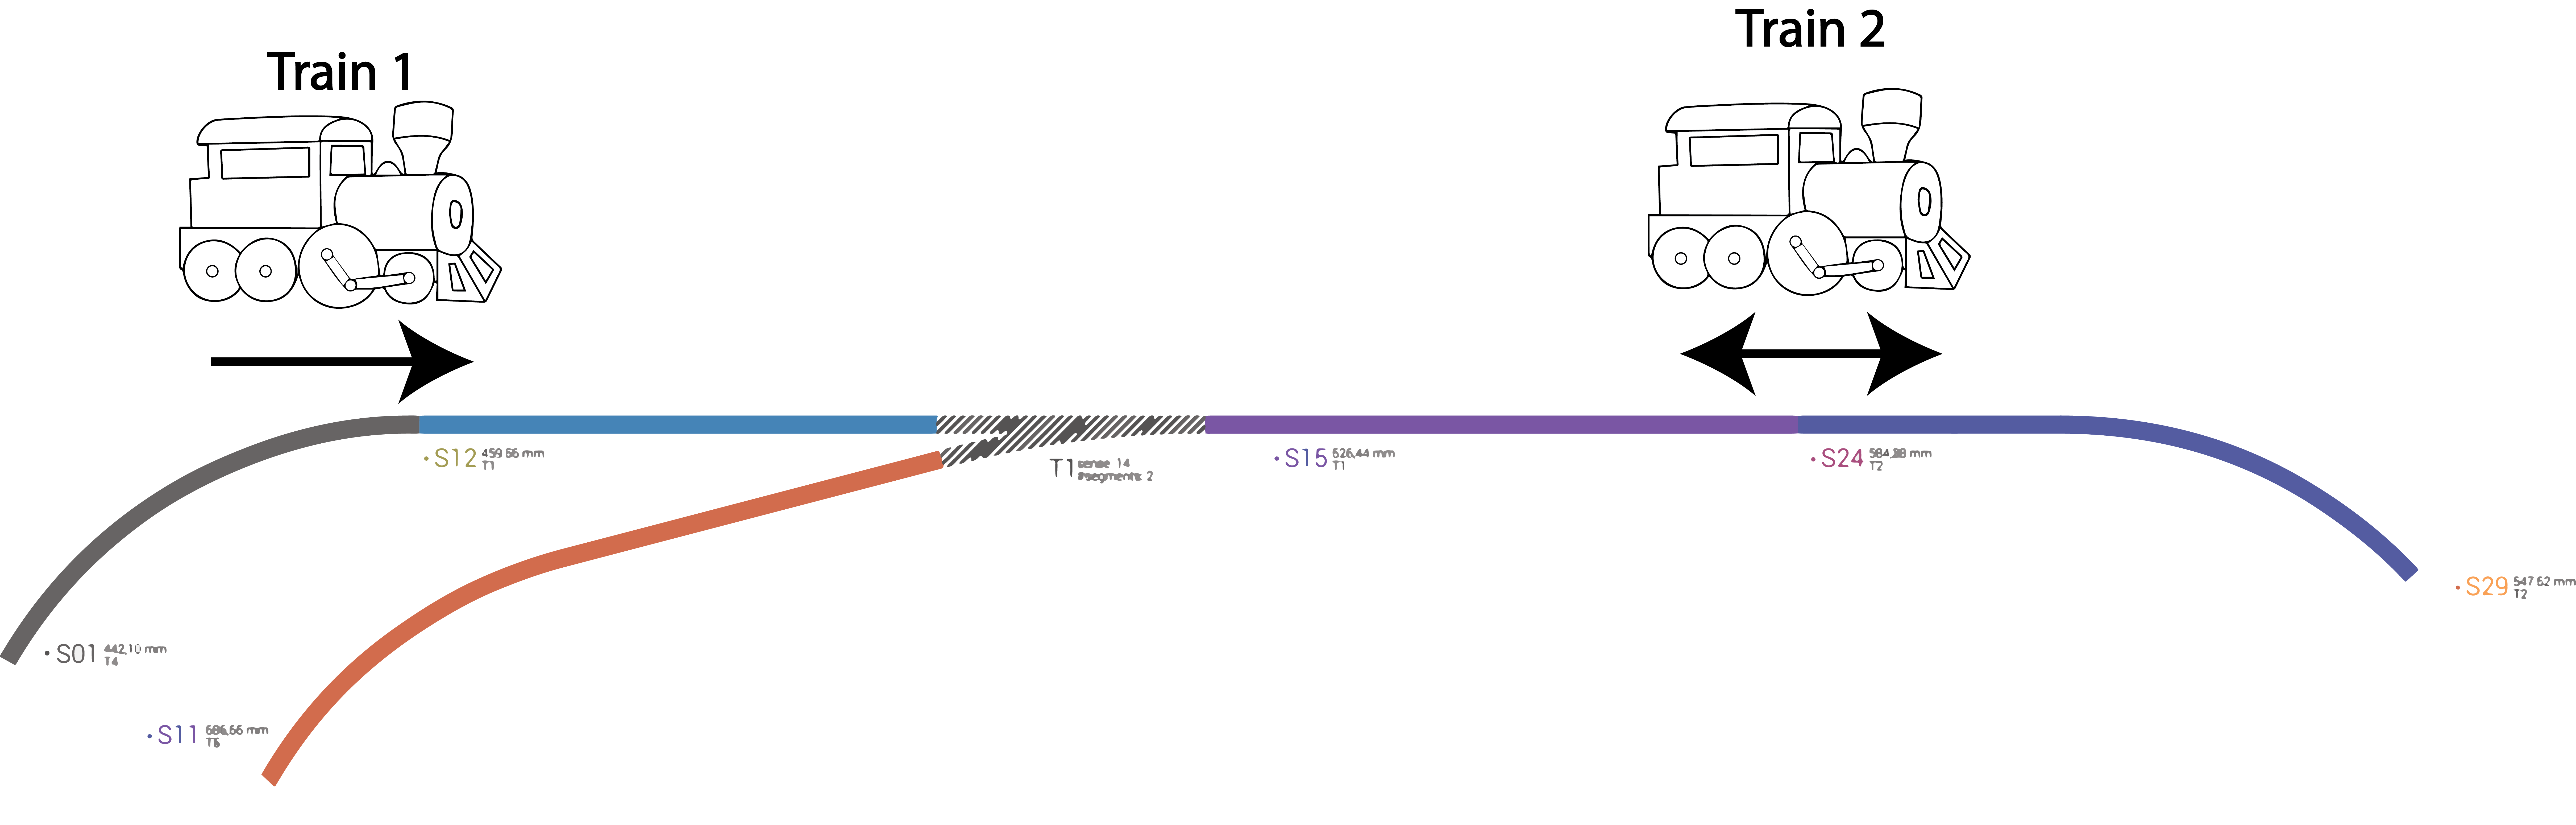
\includegraphics[width=150mm, keepaspectratio]{figures/modes3/layoutT1-scenario2.png}
	\caption{Turnout 1 collision }
	\label{fig:LayoutT1-scenario1}
\end{figure}

\paragraph{Turnout derail scenarios}
It is an unsafe situation, if train is approaching a turnout from the straight/divergent edge, but the turnout is set in the other (divergent/straight) state. On the \autoref{fig:turnout_derails}, the 2 possible derail situation is shown. In the upper case, the turnout is in state direction and any train from the straight branch will go off the rails. In addition the second case is the opposite of the previous one, that any train from the divergent branch will cut the turnout which is in straight state.
\begin{figure}[ht]
	\centering
	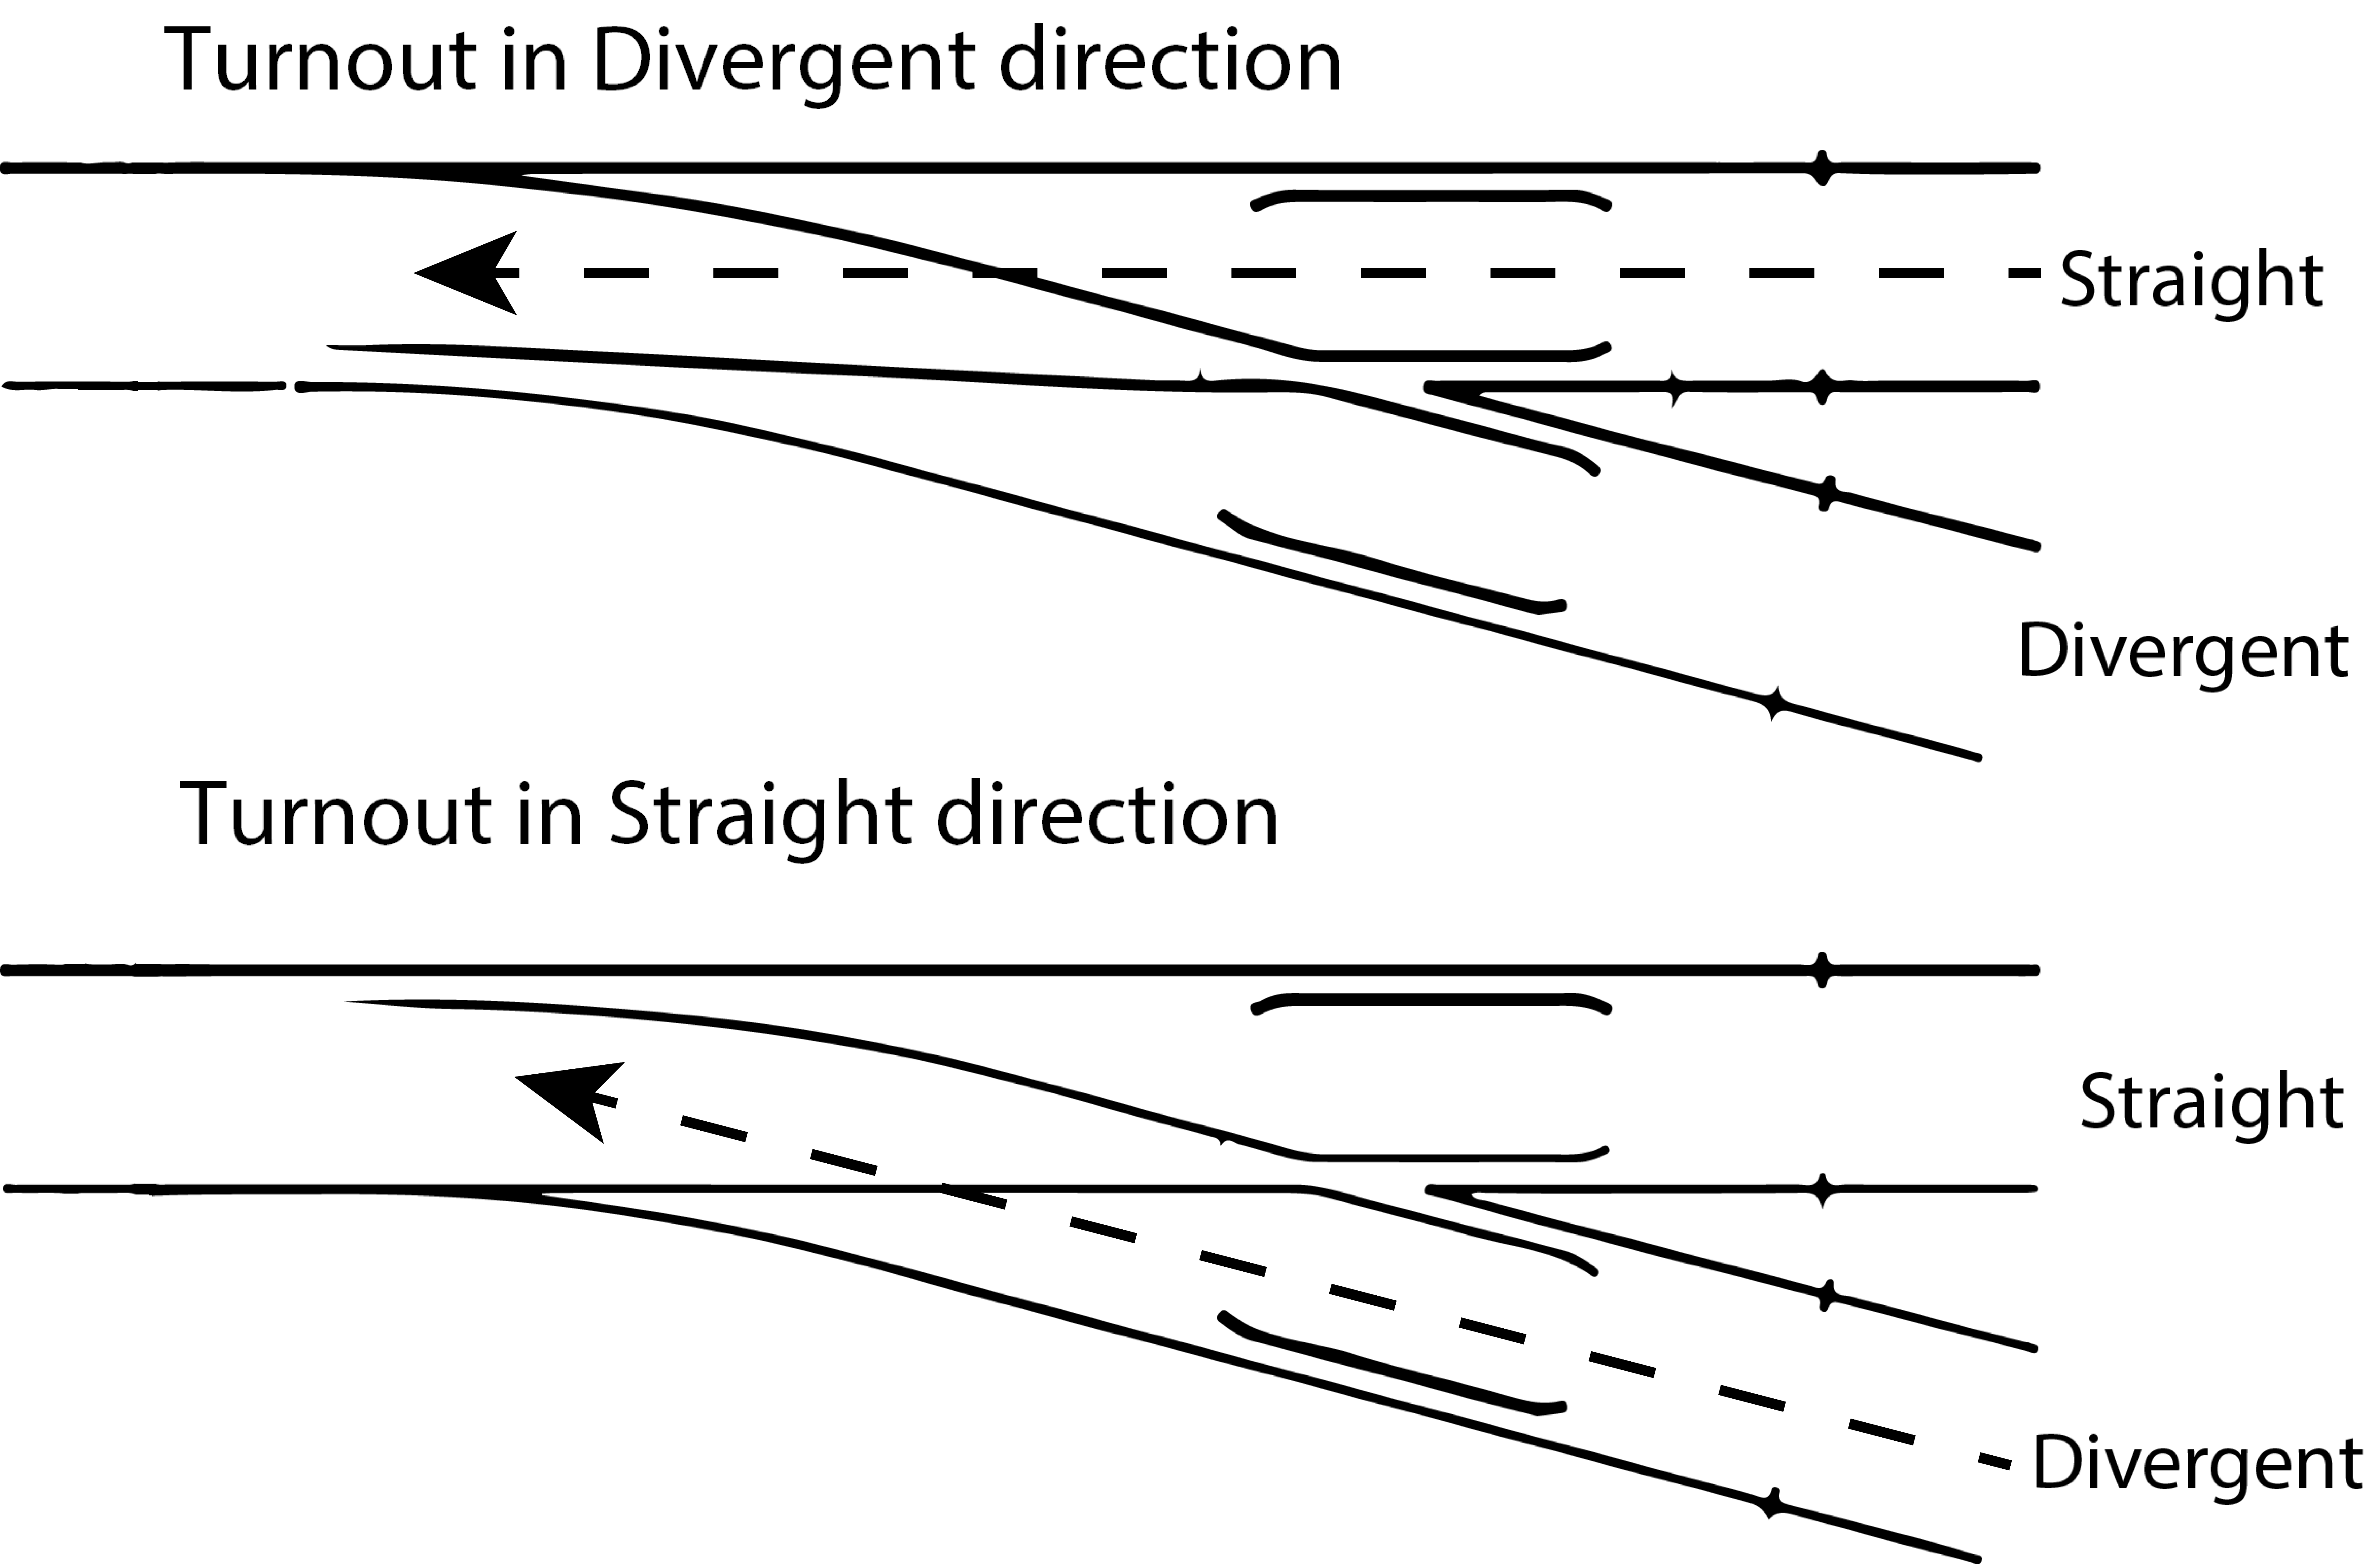
\includegraphics[width=100mm, keepaspectratio]{figures/modes3/turnout_derail.png}
	\caption{Turnout derail}
	\label{fig:turnout_derails}
\end{figure}

\section{MoDeS$^3$ Requirements}\label{section:REQ}
In this section I want to collect the requirements for the above described software and hardware extension elements in the system, not considering market products. I have categorized them into functional and component groups.

\todo[inline]{Create sysml diagrams for better overview}

\paragraph{Hardware extensions}
\begin{enumerate}[label=REQ-BBB-\arabic*, leftmargin=*, format=\small]
	\item The BeagleBone Black cape must supply 5VDC power source.
	\item The BeagleBone Black expander must provide further options to attach additional hardware elements. The purpose is to access application processor and PRU unit pins of BeagleBone Black with more elements.
\end{enumerate}

\begin{enumerate}[label=REQ-SA-\arabic*, leftmargin=*, format=\small]
	\item The Segment actuator must stop the train on the given section with the built in \textit{Command Station} (see section \ref{basics:CS}).
\end{enumerate}

\begin{enumerate}[label=REQ-TA-\arabic*, leftmargin=*, format=\small]
	\item The Turnout actuator must switch the corresponding turnout between divergent and straight states.
	\item The Turnout actuator must sense the actual state of the connected turnout.
\end{enumerate}

\paragraph{Occupancy detection software elements}
\begin{enumerate}[label=REQ-SOQ-\arabic*, leftmargin=*, format=\small]
	\item The Section Occupancy Query must collect and store the occupancy information about all segments on the track. \label{req:SOQ}
\end{enumerate}

\begin{enumerate}[label=REQ-OCQ-\arabic*, leftmargin=*, format=\small] 
	\item The Occupancy Query software element must determine whether a train is on a specific segment (results a free occupancy state) or not (results an occupied occupancy state) for each segment.  \label{req:OCQ-1}
	\item The Occupancy Query software element must send a message when an occupancy state changed for any segment. The component must send all the other current section's occupancy states in this message. \label{req:OCQ-2}
\end{enumerate}

\paragraph{Track segment controller software elements}
\begin{enumerate}[label=REQ-GPIO-\arabic*, leftmargin=*, format=\small] 
	\item The GPIO software element must be able to change the GPIO pins between their input and output states. \label{req:GPIO-1}
	\item The GPIO software element must be able to read the connected GPIO pins. \label{req:GPIO-2}
\end{enumerate}

\begin{enumerate}[label=REQ-TEC-\arabic*, leftmargin=*, format=\small]
	\item The Track Element Controller must be able to enable and disable each section with a specific command. \label{req:TEC-1}
	\item The Track Element Controller must be able to change each turnout's direction to straight or divergent state. \label{req:TEC-2}
\end{enumerate}

\paragraph{Track control and supervisor software elements}
\begin{enumerate}[label=REQ-DB-\arabic*, leftmargin=*, format=\small]
	\item The Dashboard must observe the track element states throughout the whole life-cycle. \label{req:DB-1}
	\item The Dashboard must be able to change all turnout states. \label{req:DB-2}
	\item The Dashboard must be able to change each turnout state separately. \label{req:DB-3}
	\item The Dashboard must be able to enable and disable all segments on the track. \label{req:DB-4}
	\item The Dashboard must be able to enable and disable each segment on the track, separately. \label{req:DB-5}
\end{enumerate}

\begin{enumerate}[label=REQ-SL-\arabic*, leftmargin=*, format=\small]
	\item The Safety Logic software must stop the whole track itself, when 2 trains are in a distance of 3 segments or less. \label{req:SL-1}
	\item The Safety Logic must ensure that a train must not go on a disabled segment. \label{req:SL-2}
	\item The Safety Logic must ensure that a train must stop in the straight direction of the turnout, when the turnout is in divergent state. \label{req:SL-3}
	\item The Safety Logic must ensure that a train must stop in the divergent direction of the turnout, when the turnout is in straight state. \label{req:SL-4}
\end{enumerate}
